\documentclass[11pt,a4paper]{article}

\usepackage[T1]{fontenc}
\usepackage[utf8]{inputenc}
\usepackage[margin=2.5cm]{geometry}
\usepackage{amsmath,amssymb}
\usepackage{graphicx}
\usepackage[dvipsnames]{xcolor}

\usepackage[colorlinks,bookmarksopen,bookmarksnumbered,citecolor=CadetBlue,urlcolor=CadetBlue]{hyperref}
\usepackage{url,apacite}
\usepackage{booktabs}

\usepackage{varwidth}
\setlength{\marginparwidth}{2cm}
\usepackage[colorinlistoftodos]{todonotes}
\makeatletter
\tikzstyle{diaanotestyle} = [
    draw=\@todonotes@currentbordercolor,
    fill=\@todonotes@currentbackgroundcolor,
    line width=0.5pt,
    inner sep = 0.8 ex,
    rounded corners=4pt,align=left,
   ]

\renewcommand{\@todonotes@drawInlineNote}{%
        {\begin{tikzpicture}[remember picture,baseline={(0,0)}]%
            \draw node[diaanotestyle,font=\@todonotes@sizecommand,anchor=base west]{%
               \begin{varwidth}[t]{5cm}
                \raggedright
                \if@todonotes@authorgiven%
                    {\@todonotes@sizecommand \@todonotes@author:\,\@todonotes@text}%
                \else%
                    {\@todonotes@sizecommand \@todonotes@text}%
                \fi
                \end{varwidth}};%
            \end{tikzpicture}}%
       }%
\makeatother  

\newcommand{\asb}[1]{\textcolor{red}{#1}}

\title{Empirical critical values for Rasch item fit statistics}

\author{%
    Karl Bang Christensen$^{1}$, Ann-Sophie Buchardt$^{2}$, and Mike Horton$^{3}$\\[2ex]
    \normalsize $^{1}$Section of Biostatistics, Department of Public Health, University of Copenhagen, Denmark\\
    \normalsize $^{2}$Mary Elizabeth’s Hospital, University Hospital Copenhagen, Rigshospitalet, Denmark\\
    \normalsize $^{3}$Psychometric Laboratory for Health Sciences, University of Leeds, UK\\[2ex]
    \normalsize Corresponding author: Karl Bang Christensen, Section of Biostatistics,\\
    \normalsize Department of Public Health, University of Copenhagen,\\
    \normalsize Øster Farimagsgade 5 opg. B, 1353 København K, Denmark. Email: \texttt{kach@sund.ku.dk}
}
\date{}

\begin{document}

\maketitle

\listoftodos

\begin{abstract}
Item fit statistics are frequently reported as part of Rasch-based scale validation studies, but several commonly used statistics have unknown asymptotic distributions.
Extensive simulation studies have shown that it is not possible to provide critical fit range values that will apply in all settings. Consequently, fixed rule-of-thumb critical values may not provide the intended Type~I error rates across different sample sizes, test lengths, and other characteristics of the data. 
We propose a general approach for deriving empirical critical values under the conditions of a particular data set using parametric bootstrap. By estimating the sampling distributions of the minimum and maximum item fit statistics across all items, the approach accounts for the simultaneous evaluation of multiple items. We illustrate the approach for commonly used residual-based item fit statistics under the dichotomous Rasch model using data from the Abbreviated Mental Test Score. 
The method is implemented in the R package \texttt{RASCHplot} and in a freely available online interface. Empirical critical values provide a practical alternative to fixed rule-of-thumb cut-offs for interpreting commonly reported Rasch item fit statistics.
\end{abstract}

\noindent\textbf{Keywords:} dichotomous Rasch model, item fit, type I error, asymptotic distribution.

\section{Introduction}

Item fit is arguably one of the most relevant, and certainly the most commonly reported, feature in Rasch validation studies. In the Rasch model, the fit of an item refers to the extent to which an item functions as intended within the context of the overall measurement scale, that is, the extent to which the observed responses to the item are consistent with those expected under the model. Item fit can be evaluated in several ways, including statistical tests, standardised residuals, and graphical methods. Statistical tests typically provide a $p$-value for the hypothesis of item fit, whereas standardised residuals can be compared across items. Furthermore, graphical methods have always been an important part of Rasch analysis, for example through visual comparison of observed and expected responses.

\subsection{Background}

A very wide range of item fit statistics have been developed, but very few are used in practice. The most widely used item fit statistics are (i) the infit and outfit mean square (MNSQ) item fit statistics \cite{wright-Stone-1979,Wright-Masters-1982} reported in Winsteps \cite{Winsteps}, and (ii) the fit residual, Chi-square, and ANOVA item fit statistics reported in RUMM2030 \cite{Andrich-Sheridan-Luo-2010}. These item fit statistics are based on residuals computed for each person-item interaction, and rely on assumptions about convergence to an asymptotic distribution of the sum of squared Pearson-type standardised residuals. This has been criticised by Karabatsos \cite{Karabatsos-2000}, who provided a critical analysis of the residual fit statistics of the Rasch model and argued:

\begin{quote}
`The faulty statistical properties of the residual fit statistics do not allow either a convenient or a straightforward approach to Rasch fit analysis.'
\end{quote}

More specifically, in mathematical statistics, this assumption from linear models is known to be problematic for non-linear models like the Rasch model, because the residuals have a discrete distribution that depend on the observed value. A consequence is that each residual has a unique distribution. In this setting, it is not appropriate to claim that standardised residuals are asymptotically normal or chi-squared \cite{Jennings-1986}. 
Consequently, the theoretical reference distributions and conventional critical values used to interpret these statistics may not provide the intended Type I error rates. 

Regarding mean squared item residuals, which should ideally be close to 1.0, commonly cited recommendations vary. Bond and Fox \citeyear{Bond-Fox2015} provide rule-of-thumb ranges from 0.8-1.2 to 0.5-1.7, while Linacre \citeyear{Linacre2002} suggests 0.5-1.5 as “productive for measurement” (sic). Simple rule-of-thumb critical values for acceptable fit may, however, be inappropriate \cite{Smith-et-al-1998,Wang-Chen-2005}. Critical ranges set using adapted values such as $1\pm6/\sqrt{N}$ and $1\pm2/\sqrt{N}$ are sometimes recommended, as is the use of the Wilson-Hilferty cube-root transformation, but simulation studies show that these do not apply in all settings. In particular, MNSQ values vary across sample sizes, and maximum and minimum values are not necessarily symmetric around unity. For outfit in the case of sample sizes around 200, for example, the maximum value could be as large as 2.5, invalidating commonly used critical ranges \cite{Wang-Chen-2005,Seol2016}. Hodge and Morgan \citeyear{Hodge-Morgan-2017} similarly evaluated the stability of infit and outfit "rule-of-thumb" critical values (e.g., 0.7-1.3) in a high-stakes clinical certification exam. Comparing empirical fit statistics with 250 simulated datasets, they found that substantially more values fell within the rule-of-thumb range than within the simulated confidence intervals. This suggests that relying solely on fixed critical values can lead to incorrect conclusions about model-data fit.

Monte Carlo methods have also been used directly in the calculation of item fit statistics. Stone \citeyear{Stone-2000} described a fit statistic based on Monte Carlo that closely approximates a scaled chi-squared random variable and is similar to Yen's \citeyear{Yen-1981} method. Similar methodology was discussed by \citeA{Su-Sheu-Wang-2007}, and Wolfe \citeyear{Wolfe-2008} describes an implementation in SAS for estimating critical values for, among other things, the item fit statistics produced by the Winsteps program. Wolfe \citeyear{Wolfe-2013} subsequently examined the distributions of outfit and infit statistics under a limited number of conditions, and recommended bootstrapping to get adequate critical values. 

This raises a practical question for Rasch validation studies: under what conditions can commonly used critical values be relied upon, and when should they be replaced by empirically derived values? Instead of tabulating critical values for a wide range of conditions, we outline a general approach for the evaluation of item fit and illustrate an implementation in R for the Rasch \citeyear{Rasch-1960} model for dichotomous items (RMD). We study the behaviour of the most widely used item fit statistics under the Rasch model to see when they produce empirical Type I error rates that are close to the nominal 5\%, leading to recommendations regarding reasonable critical values under the conditions of a particular analysis. We do so in a way that reflects the way most users approach evaluation of item fit, i.e.\ looking at the evidence for all items and then evaluating whether the item that has the worst fit is a cause for concern when taking the total number of items into account. Thus, we provide guidelines for the evaluation of item fit that address the issue of multiple testing.

\subsection{Statistical framework}

Let $X_{vi} \in \{0,1\}$ denote a dichotomous random variable representing a response from person $v = 1,\ldots, N$ to item $i = 1,\ldots,K$. The simplest parametric IRT model is the Rasch \citeyear{Rasch-1960} model for dichotomous items (RMD), also known as the 1PL model, 
\begin{equation}
\label{RMD}
P(X_{vi}=x|\theta_v=\theta)
=\frac{\exp(x(\theta-\delta_i))}{1 + \exp(x(\theta-\delta_i))}.
\end{equation}

In the Rasch model the parameters $\delta_1,\ldots,\delta_k$ that can be interpreted as item difficulties and estimates $\hat\delta_1,\ldots,\hat\delta_k$ can be computed in several ways \cite{Christensen-2013,Robitzsch-2021}, but typically the choice of estimation procedure is dictated by the choice of software. For users of proprietary software this means: marginal maximum likelihood (MML) estimation for ConQuest \cite{Adams-Wu-Cloney-Wilson-2020} users; pairwise conditional estimation (PCML; \citeNP{Zwinderman-1995,Andrich-Luo-2003}) for RUMM \cite{Andrich-Sheridan-Luo-2010} users; joint maximum likelihood (JML) estimation for Winsteps \cite{Winsteps} users. 

Estimates $\hat\theta_1,\ldots,\hat\theta_N$ of the person parameters $\theta_1,\ldots,\theta_N$ can be computed using maximum likelihood (ML), weighted maximum likelihood (WML; \citeNP{Warm-1989}) and other methods \cite{Kreiner-Christensen-2013}. Again, the choice of estimator is often dictated by the choice of software.

After observing data $(x_{vi})$ and estimating item and person parameters, the issue of model fit boils down to whether or not the observed data is consistent with the data generating mechanism

\begin{equation}
\label{IRThat}
P(X_{vi}=x_{vi}|\theta_v=\hat\theta_v),
\end{equation}
for all $v = 1,\ldots,N$.

This question is typically addressed using statistical tests and tests with a specified alternative, e.g., 'misfit is due to item $i_0$', are usually used.

Let for $v=1,\ldots,N$ and $i=1,\ldots,K$
$$
E_{vi} = E(X_{vi} | \theta_v = \hat\theta_v)
$$ 
and 
$$
V_{vi} = V(X_{vi} | \theta_v = \hat\theta_v)
$$
denote the expected value and variance, respectively, of the item responses conditional on the estimated value $\hat\theta_v$ of $\theta_v$.

Let $z_{vi}$ denote the standardised residuals, that is,
$$
z_{vi} = \frac{x_{vi} - E_{vi}}{\sqrt{V_{vi}}}
$$

\subsection{Outfit and infit}

The outfit item fit statistic for the $i=1,\ldots,K$ items is defined as

\begin{equation}
u_i = \frac1N\sum_{v=1}^N z_{vi}^2.
\label{outfit}
\end{equation}

The infit item fit statistic for the $i=1,\ldots,k$ items is defined as

\begin{equation}
v_i = \frac{\sum_{v=1}^Nz_{vi}^2}{\sum_{v = 1}^N V_{vi}}.
\label{infit}    
\end{equation}

The item fit statistics (\ref{infit}) and (\ref{outfit}) have no established null distribution, although false claims that they do can be found in the early Rasch literature \cite{Wright-Panchapakesan-1969,wright-Stone-1979}. Transformations have been proposed and implemented.

\subsection{Transformations}

Let for $i=1,\ldots,K$
$$
q_i^2 = \frac{1}{N^2} \sum_{v=1}^N \frac{C_{vi}}{V_{vi}^2} - \frac1N,
$$
where
$$
C_{vi} = E_{vi}^4 (1 - E_{vi}) + (1-E_{vi})^4 E_{vi}.
$$

It has been suggested that the Wilson-Hilferty \citeyear{Wilson-Hilferty-1931} cube-root transformations
\begin{equation}\label{wilson-hilferty-OUT}
t_{u,i} = \frac{3u_i^{\frac{1}{3}} - 1}{q_i} + \frac{q_i}{3}
\end{equation}
and
\begin{equation}\label{wilson-hilferty-IN}
t_{v,i} = \frac{3v_i^{\frac{1}{3}} - 1}{q_i} + \frac{q_i}{3}
\end{equation}
yield distributions that approximate a $t$ distribution \cite[Table 5.4a, p.100]{Wright-Masters-1982}. However, this claim rests on the false assumption that the item fit statistics (\ref{infit}) and (\ref{outfit}) follow a $\chi^2$ distribution. 

Another transformation of the outfit test statistic is reported in the software package RUMM \cite{Andrich-Sheridan-Luo-2010}. This transformation is based on using the ratio $S_i/f$ where
\begin{equation}
S_i = \sum_{v = 1}^N z_{vi}^2.
\label{S}
\end{equation}
This ratio is argued to be approximately chi-square distributed on $f$ degrees of freedom using an ad hoc derivation that, in the notation of this paper, amounts to $N\cdot k$ data points minus $N+k-1$ estimated parameters with each item contributing equally yielding $f=(Nk-N-k+1)/k$. Using the approximation
\begin{equation}
V(\log(S_i/f))\simeq\frac1{f^2}{V(S_i)}
\end{equation}
the test statistic FitResid defined as 
\begin{equation}
s_i=\frac{\log(S_i/f)}{\sqrt{V(\log(S_i/f))}}
=\frac{f(\log(S_i)-\log(f))}{\sqrt{V(S_i)}}
\label{FitResid}
\end{equation}
is argued to have a symmetrical distribution with mean zero and variance one. The item fit residual is considered to be sensitive towards a deviation from the requirement of equal discrimination, and $\pm2.5$ are commonly accepted thresholds. 

\subsection{Other item fit statistics}

The McKinley and Mills \citeyear{McKinley-Mills-1985} likelihood ratio $G^2$ and Yen's \citeyear{Yen-1981} Q1 have both been argued to have an approximate $\chi^2$ distribution. Computing one of these fit statistics for each of the $K$ items and reporting the largest observed value will inherently lead to type I errors. 

The Molenaar \citeyear{Molenaar-1983} item fit statistic $U$ for evaluating item fit in the RMD summarizes trends in residuals calculated in different score groups derived by partitioning the score range into three intervals. Molenaar argued that $U$ has an asymptotic standardised normal distribution under the Rasch model and that large positive or negative values for an item indicates that the discrimination is stronger or weaker, respectively, than what is assumed by the Rasch model.

\paragraph{}
Published Rasch validation studies will very often report an item fit statistic for each of the items in a scale and then report on the item (or items). Trust in the null distribution and a reasonable strategy for addressing multiple testing is needed. 

\section{Methods}

Inspired by earlier work \cite{Stone-2000,Su-Sheu-Wang-2007,Wolfe-2008,Hodge-Morgan-2017} we propose the following general approach based on empirical cirtical values obtained from simulated data.

\subsection{Empirical critical values}

\begin{enumerate}
\item Given estimates of $\delta_1,\ldots,\delta_K$ and $\theta_1,\ldots,\theta_N$ simulate $B$ data sets using the data generating mechanism (\ref{IRThat}) and, for each of these:
\begin{enumerate}
\item Estimate the values of $\delta_1^{(s)},\ldots,\delta_K^{(s)}$ and the values of $\theta_1^{(s)},\ldots,\theta_N^{(s)}$ using an estimation method of choice;
\item Using the parameter estimates, compute the item fit statistic of choice $Z_i^{(s)}$ for each item;
\item compute $L^{(s)}=\min\{Z_i^{(s)}:i=1,\ldots,K\}$; and
\item compute $U^{(s)}=\max\{Z_i^{(s)}:i=1,\ldots,K\}$.
\end{enumerate}
\item Evaluate percentiles for $(L^{(s)})_{s=1,\ldots,B}$, $(U^{(s)})_{s=1,\ldots,B}$, or both, as appropriate.
\end{enumerate}

This approach applies to any estimation method and, for this reason, can be used to study the empirical distribution of item fit statistics from proprietary software. 

\subsection{Implementation for the Rasch model for dichotomous items}

The computational algorithm relies on repeated random sampling to obtain a sampling distribution for an item fit statistic of interest, in particular, the outfit, infit, or item fit residual. From the imported item and person parameter estimates $\hat\delta_1,\ldots,\hat\delta_k$ and $\hat\theta_1,\ldots,\hat\theta_k$ conditional probabilities for item responses are computed under the model \eqref{RMD}. The probabilities are stored in a matrix as follows:

\begin{equation}
\boldsymbol{\hat{P}}=\left[\hat{P}_{vi}\right]_{\substack{v=1,\ldots,N \\ i=1,\ldots,K}}=\left[P(x_{vi}=1 \mid \theta_v=\hat\theta_v; \delta_i=\hat\delta_i)\right]_{\substack{v=1,\ldots,N \\ i=1,\ldots,K}}.
\label{probability-matrix}
\end{equation}

Then, for each cell in the matrix of probabilities, a random number is generated from a uniform distribution $p^{(l)}_{vi} \sim \mathcal{U}[0,1]$ and we define $x^{(l)}_{vi}=1$ if $\hat{P}_{vi} > p^{(l)}_{vi}$ and $x^{(l)}_{vi}=0$ otherwise. This way we generate a data matrix  $\mathbf{x}^{(l)}$, $l=1,2,\ldots$, of item responses. For each sample, we estimate the parameters of a parametric IRT model using the estimation methods applied to the observed data to reproduce the conditions of the original analysis; the same methods used to estimate the item and person parameters in the observed data should also be used for each simulated data set. Furthermore, the item fit statistics presented above are computed. Finally, from a suitable number of repetitions, we obtain an estimate of the sampling distribution for the minimum and maximum item fit statistics, $(L^{(s)})_{s=1,\ldots,B}$ and $(U^{(s)})_{s=1,\ldots,B}$, respectively. 
Four estimation  methods are available for the item parameter estimation through the \texttt{RASCHplot} package, namely, PCML \cite{sirt}, CML \cite{erm}, JML  \cite{tam}, and MML \cite{tam}. Two estimation methods are available for the person parameter estimation, namely WML and ML \cite{sirt}. 

\subsection{Implementation for the Rasch model for polytomous items}

For ease of presentation, the main text of this work discusses only the Rasch model for dichotomous items. Everything generalizes to the Rasch model for polytomous items (Appendix

\subsection{Software implementation}

The proposed method is implemented in the \texttt{RASCHplot} package which is available as a free package for the R software environment \cite{R}. 
The implementation generates empirical sampling distributions of the $(L^{(s)})_{s=1,\ldots,B}$ or maximum $(U^{(s)})_{s=1,\ldots,B}$ values of the item fit statistic of interest.
This is possible for any of the item fit statistics presented above. 
These distributions can be visualised using density plots, with percentiles representing empirical critical values indicated in the figures. For example, the values 2.5\% and 5\% could be reasonable for the minimum while 95\% and 97.5\% could be reasonable for the maximum. 

To make the method available without requiring users to code in R, we have supplemented the R implementation with the \texttt{RMDitemfit} Shiny app \cite{shiny}. Shiny is an open source R package that provides an elegant and powerful web framework for building web applications using R \cite{beeley2013}. The app allows users to generate sampling distributions for different Rasch item fit statistics using user-specified settings and to visualize the resulting empirical critical values. The app is available free of charge (\url{https://shiny.sund.ku.dk/RMDitemfit/}) and can also be run locally through the \texttt{RASCHplot} package using \texttt{RASCHplot::app("RMDitemfit")}.


\section{Example: Abbreviated Mental Test Score}

This example uses the responses of 197 persons to the ten questions of the Abbreviated Mental Test Score \cite[AMTS]{hodkinson72}. One point is given for each correct answer; a score of 6 or less suggests that the patient has some mental impairment. Table \ref{tab:amtsfit} shows the item locations and three item fit statistics for the ten items.

\begin{table}[h!]
    \centering
    \caption{Item locations and three item-fit evaluations for the abbreviated mental test score.} \label{tab:amtsfit}
    \begin{tabular}{lrrrrr}
    \\
    \toprule
             &          &    & RUMM     & \multicolumn{2}{c}{Winsteps}\\
    Item     & $\delta$ & SE & FitResid & Outfit & Infit\\
    \midrule
    Age      & -0.68 & 0.22 & -1.27 & 0.63 & 0.84 \\
    Time     &  0.08 & 0.20 &  0.57 & 1.00 & 0.98 \\
    Address  &  1.91 & 0.20 &  0.62 & 1.05 & 1.12 \\
    Name     & -0.62 & 0.22 & -0.65 & 0.75 & 0.87 \\
    Year     &  0.16 & 0.20 & -1.30 & 0.70 & 0.85 \\
    Dob      & -1.69 & 0.27 & -0.46 & 0.72 & 0.99 \\
    Month    &  0.46 & 0.20 & -2.65 & 0.57 & 0.66 \\
    Firstww  & -0.12 & 0.21 &  1.35 & 1.18 & 1.14 \\
    Monarch  &  0.17 & 0.20 & -0.28 & 0.85 & 0.93 \\
    Countbac &  0.34 & 0.20 &  2.30 & 1.34 & 1.25 \\
    \bottomrule
    \end{tabular}
\end{table}

For all three fit statistics, the smallest value is observed for the item 'Month' and the largest for the item 'Countbac'. Thus, the three fit statistics agree in identifying the items with the most extreme values. With respect to `Month', this is also consistent with an earlier reported analysis using comparison of observed and expected item-restscore correlations \cite{Christensen-Kreiner-2013} and graphical evaluation of item fit \cite{Buchardt2023VisualizingR}. 

\subsection{FitResid}

Conventional rules-of-thumb would flag the item 'Month', with an observed fit residual of $-2.65$, as an anomaly. However, minimum values below $-2.65$ occurred in 16\% of the simulated data sets, and the observed value therefore does not constitute evidence against the Rasch model. In contrast, maximum values above the observed value of 2.30 for 'Countbac' occurred in only 1\% of the simulated data sets, suggesting evidence against the Rasch model. 

\autoref{fig:amtsFitResidMinMax} shows the empirical distribution of the smallest (left panel) and largest (right panel) values of the ten FitResid values computed in each of $B=2000$ simulated data sets. 

\begin{figure}[h!]
    \centering
    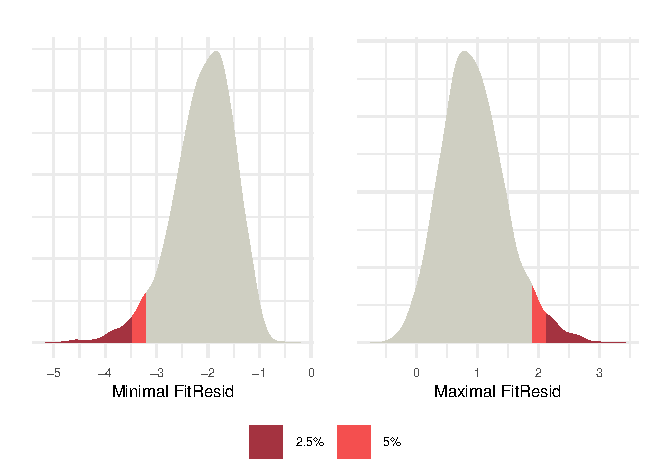
\includegraphics{amtsFitResid.pdf}
    \caption{Empirical critical values for minimum (left) and maximum (right) item fit residual values for the AMTS. Values that occur less than 5\% of the times and values that occur less than 2.5\% of the times are indicated.}
    \label{fig:amtsFitResidMinMax}
\end{figure}

Minimum values below -3.47 and -3.19 occur in 2.5\% and 5\% of the simulated data sets, respectively. Similarly, maximum values above 2.13 and 1.89 occur in 2.5\% and 5\% of the simulated data sets, respectively.

\subsection{Outfit}

For outfit, minimum values below the observed values of 0.57 for 'Month' occurred in 57\% of the simulated data sets, and the observed value therefore does not constitute evidence against the Rasch model. Maximum values above the observed value of 1.34 for 'Countbac' occurred in only  4\% of the simulated data sets, suggesting mild evidence against the Rasch model. 

\autoref{fig:amtsOutfitMinMax} shows the empirical distribution of the smallest (left panel) and largest (right panel) outfit values computed in each of $B=2000$ simulated data sets. 
The values that occur less than 5\% of the times and values that occur less than 2.5\% of the times are indicated.

\begin{figure}
    \centering
    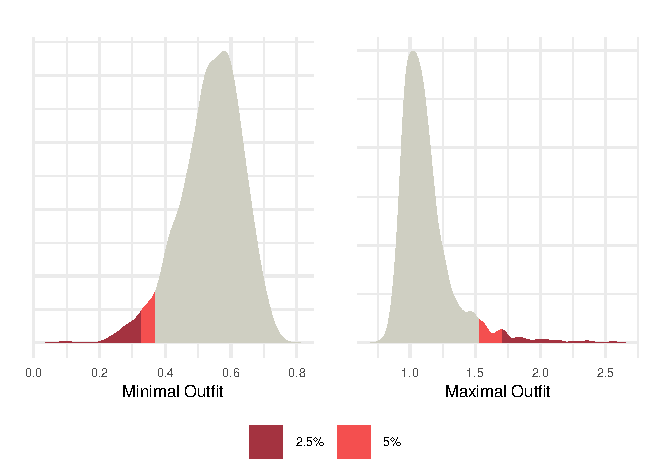
\includegraphics{amtsOutfit.pdf}
    \caption{Empirical critical values for minimum (left) and maximum (right) outfit item fit statistics for the AMTS. Values that occur less than 5\% of the times and values that occur less than 2.5\% of the times are indicated.}
    \label{fig:amtsOutfitMinMax}
\end{figure}



\subsection{Infit}

For infit, minimum values below the observed value of 0.66 for 'Month' occurred in only 1\% of the simulated data sets and thus the observed constitutes evidence against the Rasch model. Maximum values above the observed value of 1.25 for 'Countbac' occurred in only 3\% of the simulated data sets, suggesting mild evidence against the Rasch model. 

\autoref{fig:amtsInfitMinMax} shows the empirical distribution of the smallest (left panel) and largest (right panel) infit values computed in each of $B=2000$ simulated data sets. 
Again, the values that occur less than 5\% of the times and values that occur less than 2.5\% of the times are indicated.

\begin{figure}
    \centering
    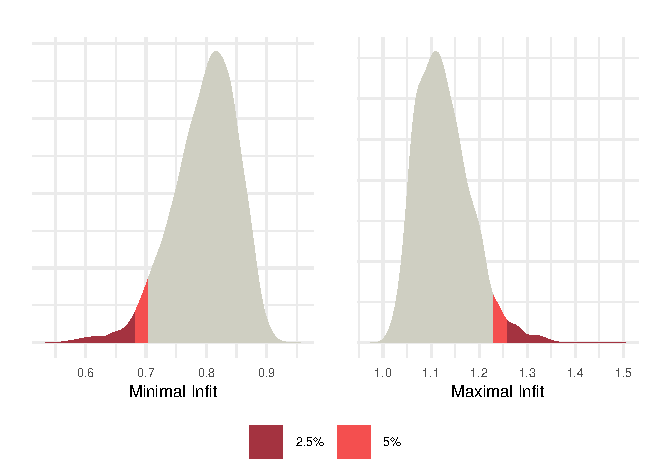
\includegraphics{amtsInfit.pdf}
    \caption{Empirical critical values for minimum (left) and maximum (right) infit item fit statistics for the AMTS. Values that occur less than 5\% of the times and values that occur less than 2.5\% of the times are indicated.}
    \label{fig:amtsInfitMinMax}
\end{figure}


\paragraph{}
The example illustrates that the interpretation of observed item fit statistics can differ substantially when empirical rather than conventional critical values are used. Although 'Month' has the smallest observed value for all three statistics, its fit residual and outfit values are not unusual under the fitted Rasch model, whereas its infit value is. Conversely, the largest values observed for 'Countbac' are relatively unusual for all three fit statistics. Thus, the same items are identified as having the most extreme observed values, but whether these values provide evidence against the Rasch model depends on the empirical distribution of the particular fit statistic.


\section{Discussion}

In this paper, we propose an approach for estimating empirical critical values for Rasch item fit statistics under the conditions of the data being analysed, rather than relying on fixed rule-of-thumb cut-offs. 
The method is implemented in R and with an accompanying online interface.

The approach uses parametric bootstrap to generate empirical distributions of the minimum and maximum item fit statistics and thereby also accounts for the multiple testing inherent in evaluating item fit across several items. The AMTS example illustrates the practical importance of this approach. An observed fit statistic that would be considered anomalous according to a conventional fixed cut-off may not be unusual under the fitted Rasch model, while values falling within or close to conventional ranges may be relatively unusual. Thus, whether an observed item fit statistic constitutes evidence against the Rasch model depends not only on its numerical value, but also on the conditions under which it was obtained.

This matters because the use of a single critical value for misfit diagnosis, applied uniformly across different conditions, leads to both the overdetection and underdetection of misfit. 

The empirical distributions of item fit statistics may depend on characteristics such as sample size, test length, response format, and targeting. For example, the standard deviations of the infit and outfit mean squares become smaller as sample size increases. Simulation studies have also shown that the means of $t$-transformed infit and outfit item fit statistics are very close to zero but have standard deviations considerably smaller than one, with the standard deviations decreasing further as the number of items increases. These findings are consistent with the critical analysis by Karabatsos \cite{Karabatsos-2000}, who demonstrated that the faulty statistical properties of residual fit statistics do not allow a simple and generally applicable approach to Rasch fit analysis.

Simulation- and bootstrap-based approaches to evaluating model fit are not new. Wolfe \citeyear{Wolfe-2013}, for example, described three implementations of the bootstrap procedure for evaluating person and item fit, and other simulation-based approaches have previously been proposed \cite{Stone-2000,Su-Sheu-Wang-2007,Hodge-Morgan-2017}. The present approach builds on this work by providing empirical critical values for the residual item fit statistics commonly reported by Rasch software and by basing these on the distributions of the minimum and maximum values across all $K$ items, and for this reason the resulting critical values account for the simultaneous evaluation of item fit across the instrument and accommodate the wide variation in the number of items across instruments. For a one-sided evaluation, the 5th percentile of the minimum or the 95th percentile of the maximum corresponds to an approximate 5\% probability of observing at least one value beyond the respective critical value under the fitted Rasch model. For a two-sided evaluation, using the 2.5th percentile of the minimum and the 97.5th percentile of the maximum allocates the nominal 5\% level between the two tails.

The proposed approach should not be interpreted as solving the statistical limitations of residual item fit statistics themselves. Alternative item fit statistics with known asymptotic properties exist \cite{Christensen-Kreiner-2013,Muller-2020,Johansson2025} and have been implemented in R \cite{iarm}. Karabatsos \cite{Karabatsos-2000} also advocated residual-free Rasch fit statistics based on the number of Guttman response errors, and for the dichotomous Rasch model Kreiner and Christensen (\citeyear{Christensen-Kreiner-2010}) studied exact tests based on the same principle. Where appropriate, methods with established statistical properties are preferable to relying on residual fit statistics with problematic or unknown null distributions.

Nevertheless, residual fit statistics remain widely used and are routinely produced by major Rasch software packages. Until item fit statistics with known asymptotic properties are more commonly used, empirical critical values provide a pragmatic way of interpreting these residual fit statistics in the context in which they were obtained. The implementation in \texttt{RASCHplot} and the \texttt{RMDitemfit} Shiny app make it possible to obtain these critical values for the conditions of a particular analysis. The online interface (Shiny app) is freely available online and does not require users to work directly in R.

\citeA{Wu-Adams-2013} examined residual-based fit statistics in the RMD and analytically illustrated that residual-based fit statistics provide a measure of the relative slope of empirical item characteristic curves. This is an argument for retaining reported values while taking extra caution when evaluating if an observed value is a statistical anomaly.


\bibliographystyle{apacite}
\bibliography{biblio.bib}

\end{document}
